 \documentclass[13pt]{article}

\usepackage{fancyhdr}

\fancypagestyle{group}{
\fancyhf{}
\rhead{گزارش فاز دوم پروژه}
\lhead{}
\rfoot{صفحه \thepage}
}


\usepackage{cite}
\usepackage{ptext}
\pagenumbering{arabic}

\usepackage[a4paper,top=3cm,left=2.5cm,right=2.5cm,bottom=2cm]{geometry}
\usepackage{graphicx}
\usepackage{amsmath,amssymb}
\usepackage{wrapfig}
\graphicspath{./}

\usepackage{setspace}
\usepackage{listings}
\linespread{1.3}
%\usepackage{multirow}
\usepackage{amsfonts}

\usepackage{xcolor}
\usepackage{hyperref}

\usepackage{listings}
\usepackage{color}

\definecolor{mygreen}{rgb}{0,0.6,0}
\definecolor{mygray}{rgb}{0.5,0.5,0.5}
\definecolor{mymauve}{rgb}{0.58,0,0.82}

\lstset{ 
	backgroundcolor=\color{white},   % choose the background color; you must add \usepackage{color} or \usepackage{xcolor}; should come as last argument
	basicstyle=\footnotesize\texttt,        % the size of the fonts that are used for the code
	breakatwhitespace=false,         % sets if automatic breaks should only happen at whitespace
	breaklines=true,                 % sets automatic line breaking
	captionpos=b,                    % sets the caption-position to bottom
	commentstyle=\color{mygreen},    % comment style
	deletekeywords={...},            % if you want to delete keywords from the given language
	escapeinside={\%*}{*)},          % if you want to add LaTeX within your code
	extendedchars=true,              % lets you use non-ASCII characters; for 8-bits encodings only, does not work with UTF-8
	firstnumber=1,                % start line enumeration with line 1000
	frame=single,	                   % adds a frame around the code
	keepspaces=true,                 % keeps spaces in text, useful for keeping indentation of code (possibly needs columns=flexible)
	keywordstyle=\color{blue},       % keyword style
	language=C,                 % the language of the code
	morekeywords={*,...},            % if you want to add more keywords to the set
	numbers=left,                    % where to put the line-numbers; possible values are (none, left, right)
	numbersep=5pt,                   % how far the line-numbers are from the code
	numberstyle=\tiny\color{mygray}, % the style that is used for the line-numbers
	rulecolor=\color{black},         % if not set, the frame-color may be changed on line-breaks within not-black text (e.g. comments (green here))
	showspaces=false,                % show spaces everywhere adding particular underscores; it overrides 'showstringspaces'
	showstringspaces=false,          % underline spaces within strings only
	showtabs=false,                  % show tabs within strings adding particular underscores
	stepnumber=2,                    % the step between two line-numbers. If it's 1, each line will be numbered
	stringstyle=\color{mymauve},     % string literal style
	tabsize=2,	                   % sets default tabsize to 2 spaces
	title=\lstname                   % show the filename of files included with \lstinputlisting; also try caption instead of title
}
\lstdefinestyle{customc}{
	belowcaptionskip=1\baselineskip,
	breaklines=true,
	frame=L,
	xleftmargin=\parindent,
	language=C,
	showstringspaces=false,
	basicstyle=\footnotesize\ttfamily,
	keywordstyle=\bfseries\color{green!40!black},
	commentstyle=\itshape\color{purple!40!black},
	identifierstyle=\color{blue},
	stringstyle=\color{orange},
}

\usepackage{enumerate}
\usepackage{ptext}
\hypersetup{colorlinks=true,linkcolor=black,urlcolor=blue}
\usepackage{caption}
\usepackage{subcaption}

\usepackage[nottoc, notlot, notlof]{tocbibind}
\usepackage{xepersian}

\settextfont[]{XBNiloofar}
\setdigitfont{Yas}
\setlatintextfont{Times New Roman}
\setlength{\parindent}{0pt}
\pagestyle{group}
\begin{document}
\fontsize{13}{14}\selectfont
\begin{titlepage}
	\centering
	\large{به نام خدا}\\
	[2cm]
	
\includegraphics[width=0.2\textwidth]{sharif-logo-fa.png}\\
	[1.5cm]
	\Huge{
		فاز دوم پروژه
	}\\[2.5cm]
	
	\huge{سیستم‌های عامل\\
	دکتر جلیلی
	}\\
	[2cm]
	\Large{
	وحید زهتاب}\\
	\large{96110067}\\
\Large{
	آروین آذرمینا}\\
\large{96105542}\\
	\Large{
	کورش شریعت}\\
	\large{96109714}\\[2.5cm]
	\large{دانشکده مهندسی کامپیوتر\\دانشگاه صنعتی شریف\\{تابستان ۱۳۹۹}}
\end{titlepage}
\begin{abstract}
	هدف این فاز پیاده‌سازی قاعده 
	\lr{No Read Up, No Write Down}
	 در لینوکس است. در این  قاعده برای هر کاربر و فایل یک سطح دسترسی امنیتی در نظر گرفته می‌شود و اجازه عملیات‌ خواندن و نوشتن با توجه به سطح دسترسی این دو صادر می‌شود. برای پیاده‌سازی این قاعده یک \textbf{ماژول کرنل} طراحی شد که جایگزین ماژول \texttt{open} شده و با دریافت سطوح امنیتی از سطح کاربر عملیات خواندن و نوشتن را کنترل می‌کند.
\end{abstract}
\hrulefill
%----------------------------------------------------- %
\section{برنامه راه‌انداز}
	این کد شامل تعدادی تابع اضافه علاوه بر توابع پایه یک ماژول می‌باشد که در ادامه  شرح داده‌شده‌اند. تنها نحوه کارکرد توابع
\texttt{device\_open device\_release}
	عینا مانند فازهای قبل است که در مستندات مربوطه بحث شده‌اند.
	 \subsection{تابع \lr{\texttt{module\_startup}} و \lr{\texttt{module\_cleanup}}}
	این تابع هنگامی صدا زده می‌شود که ماژول به کرنل اضافه شود. کارکرد این تابع رجیستر کردن ماژول است. سپس جدول syscall لود شده و پوینتر تابع 
	\texttt{open}
	به تابعی که در ماژول نوشته‌شده تغییر می‌کند. کد این دو تابع در ادامه آمده است.
	 \lstset{escapechar=@,style=customc}
	 \begin{latin}
	 	\begin{lstlisting}
static int __init module_startup(void)
{
	printk(KERN_INFO "initializing module\n");
	major_num = register_chrdev(MAJOR_NUMBER, DEVICE_NAME, &file_ops);

	sys_call_table = (sys_call_ptr_t *)kallsyms_lookup_name("sys_call_table");
	old_open = (custom_open)sys_call_table[__NR_open];

	write_cr0(read_cr0() & (~0x10000));
	sys_call_table[__NR_open] = (sys_call_ptr_t)my_open;
	write_cr0(read_cr0() | 0x10000);
	printk(KERN_INFO "open syscall was replaced\n");

	if (major_num < 0)
	{
		printk(KERN_ALERT "Could not register device: %d\n", major_num);
		return major_num;
	}
	else
	{
	printk(KERN_INFO "phase2 module loaded with device major number % d\n", major_num);
	return 0;
	}
}

static void __exit module_cleanup(void)
{
	unregister_chrdev(major_num, DEVICE_NAME);
	u_entry * cur_u = users;
	u_entry * temp_u;
	f_entry * cur_f = files;
	f_entry * temp_f;
	while(cur_u != NULL){
		temp_u = cur_u;
		cur_u = cur_u->next;
		kfree(temp_u);
	}
	while(cur_f != NULL){
		temp_f = cur_f;
		cur_f = cur_f->next;
		kfree(temp_f);
	}
	write_cr0(read_cr0() & (~0x10000));
	sys_call_table[__NR_open] = (sys_call_ptr_t)old_open;    
	write_cr0(read_cr0() | 0x10000);
	printk(KERN_INFO "open syscall was replaced with the old one\n");
	printk(KERN_INFO "phase2 module successfully unloaded\n");
}\end{lstlisting}
	 \end{latin}
 \vspace{-2\baselineskip}
 	در ابتدا در تابع 
 	\texttt{module\_startup}
 	 ماژول رجیستر شده (خط ۴). سپس آدرس تابع پیشفرض 
 	 \texttt{open}
 	 ذخیره شده و تابع اصلاح‌شده در جدول قرار می‌گیرد. جدول
 	 \lr{syscall}
 	 در صفحه‌ای از حافظه قرار دارد که به صورت 
 	 \lr{read only}
 	  است. بنابراین باید ابتدا قابلیت نوشتن فراهم شود. برای این کار از تابع 
 	  \texttt{write\_cr0}
 	  استفاده می‌شود که بیت فلگ مربوط به حافظه‌ی جدول را تغییر می‌دهد. پس از تغییر جدول، در خط ۱۱ این فلگ به حالت عادی خود باز می‌گردد. در نهایت در صورت وقوع مشکل در فرآیند ثبت ماژول پیغام خطا چاپ می‌شود.
 	  
 	  	تابع  
 	  	 \lr{\texttt{module\_cleanup}} 
 	  	نیز عملکردی عکس تابع
 	  	 \lr{\texttt{module\_startup}} 
 	  	دارد. ابتدا ماژول \\
 	  	  \lr{unregister}  
 	  	شده و متغیرهای آن از حافظه پاک می‌شوند. سپس جدول
 	  	\lr{syscall}
 	  	 به حالت قبل خود باز می‌گردد.
 	  \subsection{توابع مربوط به کاربرها و فایل‌ها}
 	  این لیست شامل توابع 
 	  \lr{\texttt{find\_user\_entry}, \texttt{find\_file\_entrt}, \texttt{add\_user}}
 	  و
 	  \texttt{add\_file}
 	  است. در واقع داده‌ساختار به‌کاربرده‌شده برای ذخیره‌سازی کاربرها و فایل‌ها یک لیست پیوندی است که شامل شناسه‌ی آنها و سطح دسترسیشان می‌شود.
 	  ساختار این لیست پیوندی به صورت زیر است:
 	  \begin{latin}
 	  	\begin{lstlisting}
 typedef struct Node
 {
	 int uid;
	 int secl;
	 struct Node *next;
 } u_entry;
 
 typedef struct Nodef
 {
	 char *path;
	 int secl;
	 struct Nodef *next;
 } f_entry;\end{lstlisting}
 	  \end{latin}
   \vspace{-2\baselineskip}
   بنابراین نقش توابع مذکور یافتن گره در لیست پیوندی و اضافه کردن به آن است. ساختار کد جستجو و پیوست کردن یک ساختار متداول برای لیست‌های‌ پیوندی است که در ادامه آمده‌است.
   \\
   این توابع در 
   $\mathcal{O}(1)$
   به لیست پیوست کرده و در 
   $\mathcal{O}(n)$
   جستجو می‌کنند.
  	\begin{latin}
  		\begin{lstlisting}
u_entry * find_user_entry( int uid ){
	u_entry * cur = users;
	while(cur != NULL){
		if(cur->uid == uid)
			break;
		cur = cur->next;
	}
	return cur;
}

void add_user(int uid, int secl)
{
	u_entry *entry = find_user_entry(uid);
	if(entry != NULL){
		entry->secl = secl;
		return;
	}
	entry = (u_entry *)kmalloc(sizeof(u_entry),GFP_KERNEL);
	if (entry == NULL)
	{
		printk(KERN_INFO "Unable to allocate user entry");
		return;
	}
	entry->next = users;
	entry->secl = secl;
	entry->uid = uid;
	users = entry;
	printk(KERN_INFO "added user entry %d: uid(%d) secl(%d)\n", ++users_count, uid, secl);
}

f_entry * find_file_entry( char * path ){
	f_entry * cur = files;
	while(cur != NULL){
		if(strcmp(path, cur->path) == 0)
			break;
		cur = cur->next;
	}
	return cur;
}

void add_file(char *path, int secl)
{   
	f_entry *entry = find_file_entry(path);
	if(entry != NULL){
		entry->secl = secl;
		return;
	}
	entry = (f_entry *)kmalloc(sizeof(f_entry), GFP_KERNEL);
	if (entry == NULL)
	{
		printk(KERN_INFO "Unable to allocate file entry");
		return;
	}
	entry->next = files;
	entry->secl = secl;
	entry->path = path;
	files = entry;
	printk(KERN_INFO "added file entry %d: path(%s) secl(%d)\n", ++files_count, path, secl);
}  		  		
  		\end{lstlisting}
  	\end{latin}
  \vspace{-2\baselineskip}
  \subsection{توابع ارتباط با سطح کاربر}
  \subsubsection{تابع \lr{\texttt{device\_write}}}
  	این تابع هنگامی صدا زده می‌شود که بر روی 
  	\lr{Device file}
  	 مقداری نوشته شود. مقدار نوشته شده شامل سه بخش است که پشت سر هم می‌آیند. اولین رقم مربوط به فلگ فایل/کاربر است. رقم بعدی سطح امنیتی ورودی است و پس از آن شناسه کاربر یا آدرس فایل می‌آید. نکته قابل‌توجه در بخش ورودی این است که آدرس فایل بایستی به صورت یک آدرس مطلق به ماژول داده شود. پس از دریافت ورودی، مقادیر به توابع 
  	 \texttt{add\_user}
   و یا
\texttt{add\_file}
 	  داده می‌شوند. قسمتی از کد که مسئول این عملیات است در ادامه آمده است.
 	    	\begin{latin}
 	  	\begin{lstlisting}
ptr = input_buffer;
while (bytes_count--)
get_user(*(ptr++), buffer++);
if (input_buffer[0] == USER_FLAG)
{
	int uid;
	sscanf(input_buffer + 2, "%d", &uid);
	add_user(uid, input_buffer[1] - '0');
}
else if (input_buffer[0] == FILE_FLAG)
{
	int i = 0, j = 0;
	for(; i < len && input_buffer[i] != '\n'; i++);
	char * path = (char *)kmalloc((i-1) * sizeof(char), GFP_KERNEL);
	for(; j < i -2; j++)
		*(path + j) = input_buffer[2 + j];
	*(path + i - 2) = '\0';
	add_file(path, input_buffer[1] - '0');
} \end{lstlisting}
 	  \end{latin}
   \vspace{-2\baselineskip}
   در خط ۴ و ۱۰ بررسی می‌شود که ورودی فایل یا کاربر است. سپس در ادامه باقی ورودی خوانده شده و به تابع مربوطه پاس داده می‌شود (خطوط ۸ و ۱۸).
 \subsubsection{تابع \lr{\texttt{device\_read}}}
 	این تابع هنگامی صدا زده می‌شود که برنامه‌ی سطح کاربر بخواهد از روی 
 	  	\lr{Device file}
 	  	بخواند. در این شرایط، ماژول لیست کامل تمامی کاربرها و فایل‌هایی که در آن ثبت‌شده است را به همراه سطح امنیتی‌شان باز می‌گرداند. کد این بخش در ادامه‌آمده است.
 	  	\begin{latin}
 	  		\begin{lstlisting}
sprintf(msg, "");
char *msg_ptr;
f_entry *cur_file = files;
u_entry *cur_user = users;
while (cur_file != NULL)
{
	sprintf(msg, "%s%d%s:", msg, cur_file->secl, cur_file->path);
	cur_file = cur_file->next;
}
if (cur_user != NULL)
{
	sprintf(msg, "%susers:", msg);
	while (cur_user != NULL)
	{
		sprintf(msg, "%s%d%d:", msg, cur_user->secl, cur_user->uid);
		cur_user = cur_user->next;
	}
}
sprintf(msg, "%s\n", msg);

/* Set the msg_ptr to the buffer */
msg_ptr = msg;
/* Put data in the buffer */
while (len-- && *msg_ptr)
put_user(*(msg_ptr++), buffer++);
kfree(msg); 	\end{lstlisting}
 	  	\end{latin}
   	\vspace{-2\baselineskip}
   	در حلقه 
   	\texttt{while}
   	 اول (خطوط ۶ تا ۹) لیست پیوندی فایل‌ها پیمایش می‌شود و تمامی اعضای آن نوشته می‌شوند. در ادامه چک می‌شود که آیا عضوی در لیست کاربرها موجود است و در صورت موجود  بودن لیست پیوندی آن پیمایش می‌شود.
   	 \subsection{تابع \texttt{open} اصلاح‌شده}
   	 این تابع درواقع تابعیست که جایگزین تابع 
   	 \texttt{open}
   	 سیستم‌عامل شده و به‌جای آن فراخوانی می‌شود. در ابتدا فایل و کاربری در خواست دسترسی به آن می‌دهد، در لیست‌های پیوندی مربوطه یافت شده و سطح دسترسی آنها مقایسه می‌گردد. اگر شی مورد نظر در لیست یافت نشد، سطح دسترسی برابر با صفر در نظر گرفته می‌شود. نهایت با مقایسه سطوح دسترسی فایل و کاربر، در صورتی که درخواست کاربر با آنها تطابق داشت، عمل 
   	 \lr{open}
   	 با فراخوانی تابع پیشفرض انجام می‌شود.
   	 \begin{latin}
   	 	\begin{lstlisting}
int write_only = flags & O_WRONLY;
int read_write = flags & O_RDWR;

if((cur_u = find_user_entry(cur_uid))!= NULL)
	secu = cur_u->secl;

if((cur_f = find_file_entry(kfilename))!= NULL){
	secf = cur_f->secl;
	log_access(kfilename, secf, cur_uid,  secu, write_only, read_write );
}

if (secu == secf)
	return old_open(filename, flags, mode);

if( secu < secf) {
	if(write_only)
		return old_open(filename, flags, mode);
	printk(KERN_INFO "read permition denied - %d(%d) %s(%d)\n",cur_uid, secu, kfilename, secf);
	return -1;
} else {
	if(!(write_only|read_write))
		return old_open(filename, flags, mode);
	printk(KERN_INFO "write permition denied - %d(%d) %s(%d)\n",cur_uid, secu, kfilename, secf);
	return -1;
}

return old_open(filename, flags, mode);\end{lstlisting}
   	 \end{latin}
    \vspace{-2\baselineskip}
    در اینجا در خطوط ۴ و ۷ عملیات جستجو انجام می‌شود و در خطوط ۱۲ الی ۲۷ با توجه به نوع عملیات (خواندن، نوشتن یا هردو) حالت‌بندی صورت می‌گیرد.
     \subsection{بخش امتیازی}
     این فاز پروژه شامل دو بخش امتیازی می‌باشد. بخش اول پیاده‌سازی این قاعده با استفاده از ماژول کرنل است که همانطور که در بخش‌های قبل توضیح داده‌شد، رویه در پیش گرفته همین می‌باشد. بخش دوم ذخیره دسترسی به فایل‌‌ها است که در ادامه شرح داده‌شده است.
     \subsubsection{تابع \texttt{file\_open}}
     به منظور ذخیره‌سازی 
     \lr{log}
     ها در فایل، ابتدا باید یک فایل ساخته و باز شود. نقش این تابع در عمل همین است.
     \begin{latin}
     	\begin{lstlisting}
struct file *file_open(const char *path, int flags, int rights) {
	struct file *filp = NULL;
	mm_segment_t oldfs;
	int err = 0;
	
	oldfs = get_fs();
	set_fs(get_ds());
	filp = filp_open(path, flags, rights);
	set_fs(oldfs);
	if (IS_ERR(filp)) {
		err = PTR_ERR(filp);
		return NULL;
	}
	return filp;
} \end{lstlisting}
     \end{latin}
 \vspace{-2\baselineskip}
     به منظور داشتن قابلیت باز کردن فایل در ابتدا بایستی 
     \lr{data segment}
      را تغییر داده و پس از باز کردن فایل آن را به حالت اولیه باز گردانیم (خطوط ۷، ۸ و ۱۰). در نهایت فایل باز شده بازگردانده می‌شود.
      \subsubsection{تابع \texttt{log\_access}}
     این تابع قسمت اصلی نوشتن فایل را بر عهده دارد. 
     \texttt{log\_access}
     هنگامی صدا زده می‌شود که جستجوی فایل در لیست پیوندی اتمام یابد (خط ۹ کد بخش تابع \texttt{open}) و در حین فراخوانی با دریافت و محاسبه زمان فعلی تاریخچه دسترسی را به فایل باز شده اضافه می‌کند. ساختار کد این تابع به شکل زیر است.
\begin{latin}
	\begin{lstlisting}
void log_access(const char * filename, int secf,  int cur_uid, int secu, int wo, int rw){
	char data[LOG_LEN];
	char timestr[80];
	struct timespec curr_tm;
	getnstimeofday(&curr_tm);
	
	sprintf(data, "uid:%d - secu: %d - filepath: %s - secf: %d - r(%d)w(%d)rw(%d) - time(%.2lu:%.2lu:%.2lu:%.6lu)\n", 
		cur_uid, secu,filename, secf, (!(wo|rw) ? 1: 0), (wo ? 1: 0), (rw ? 1: 0), (curr_tm.tv_sec / 3600) % (24),
		(curr_tm.tv_sec / 60) % (60), curr_tm.tv_sec % 60, curr_tm.tv_nsec / 1000);
	struct file * handle =  file_open(LOG_FILE, O_WRONLY|O_CREAT|O_APPEND, 0777);
	if(handle == NULL){
		sprintf(data, "cannot open log file");
		return;
	}
	mm_segment_t oldfs;
	unsigned long long offset =0;
	oldfs = get_fs();
	set_fs(get_ds());
	vfs_write(handle, data, strlen(data), &offset);
	set_fs(oldfs);
	filp_close(handle, NULL);
)\end{lstlisting}
\end{latin}     
\vspace{-2\baselineskip}
     \section{کد سطح کاربر}
     \begin{wrapfigure}{L}{0.5\textwidth}
     	\centering
     	\vspace{-0.5cm}
     	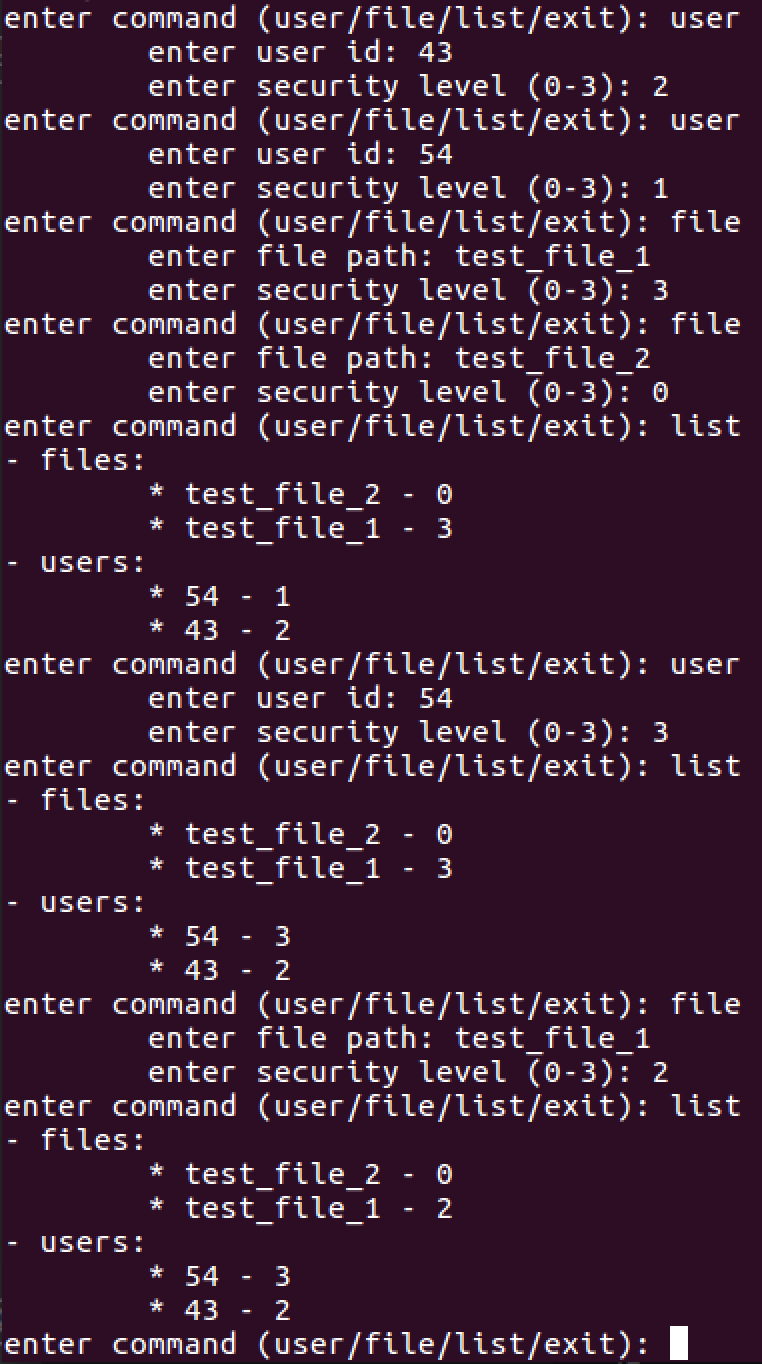
\includegraphics[width=0.45\textwidth]{screenshots/communicationWithKernel.png}
     	\caption{مثال دستورات کد سطح کاربر}
     	\vspace{-50pt}
     	\label{f1}
     \end{wrapfigure}
     علاوه بر ماژول کرنل، یک کد سطح کاربر به زبان پایتون نوشته شد که وظیفه آن مدیریت لیست سطح دسترسی برای فایل‌ها و کاربران است. نحوه کارکرد انی کد همانند فاز‌های قبلی است و ارتباط با ماژول به وسیله نوشتن و خواندن از روی
     \lr{Device file}
      صورت می‌گیرد. در این کد قابلیت‌های اضافه کردن و به‌روز رسانی فایل‌ها و کاربرها و همچنین مشاهده لیست آنها تعبیه شده‌است تا برهمکنش با لایه کرنل به سادگی صورت گیرد. نحوه کارکرد کد در شکل
      \ref{f1}
       آمده‌است . در ابتدا دو کاربر و دو فایل با سطوح دسترسی مختلف اضافه شده‌اند و سپس ذخیره‌شدن آنها نمایش داده‌شده است. در ادامه قابلیت به‌روز رسانی نشان‌ داده‌شده است. به این شکل که کاربر با شناسه \texttt{54} سطح دسترسی جدیدی پیدا کرده‌است و آن سطح دسترسی ذخیره شده‌است. این قابلیت برای فایل نیز نمایش داده‌شده است.
      \section{کامپایل ماژول}
      برای کامپایل ماژول یک \texttt{MakeFile} همانند \texttt{Makefile} فاز قبلی تنظیم شده است و با اجرای دستور \texttt{make} در ترمینال ماژول کامپایل می‌شود. در ادامه افزوده‌شدن به کرنل و 
      \lr{Major number}
      ماژول در 
      \lr{log}
      های کرنل مشهود هستند. باقی مراحل کامپایل نیز من جمله اجرای دستور 
      \lr{\texttt{make test}}
      همانند فازهای قبل هستند.
      \section{اجرا و تست برنامه}
      برای تست برنامه ابتدا تعدادی 
      \lr{entry}
      برای فایل و کاربر اضافه می‌کنیم و عملیات خواندن و نوشتن را روی آنها انجام می‌دهیم.
      \begin{figure}[h]
      	\centering
      	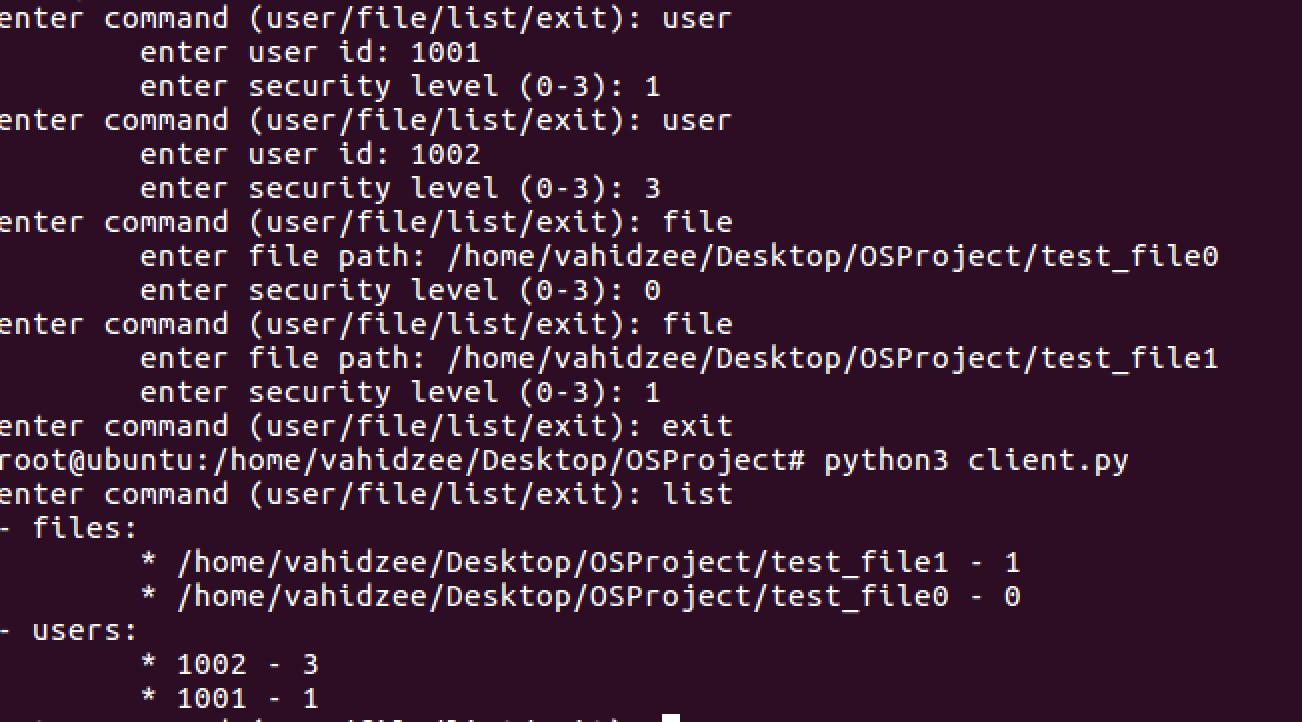
\includegraphics[width=0.8\textwidth]{screenshots/testFilesAndUsers.png}
      	\caption{افزودن کاربرها و فایل‌ها}
      \end{figure}
   \begin{figure}[h]
  	\centering
  	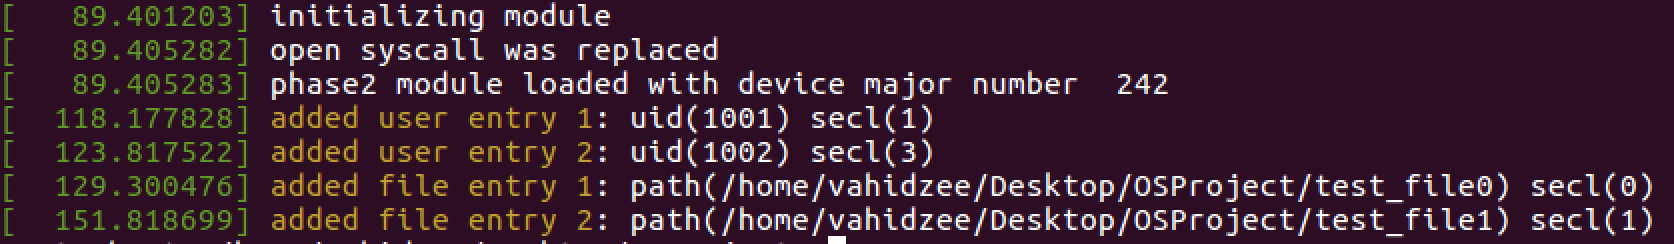
\includegraphics[width=0.8\textwidth]{screenshots/testFilesAndUsersAddedLog.png}
  	\caption{لاگ کرنل هنگام کامپایل و افزودن داده‌ها}
  \end{figure}

	در ابتدا با کاربر اولیه (دارای $1000 = \mathrm{uid}$) تعدادی فایل باز می‌کنیم. این امر با سه کد ساده C که کارشان استفاده از \texttt{open} (برای سه امر خواندن، نوشتن و خواندن/نوشتن) و پرینت کردن نتیجه عملیات است انجام شد. از آنجایی که ۱۰۰۰ در لیست ماژول وجود ندارد، به طور پیشفرض سطح امنیتی صفر به آن اختصاص می‌گیرد. بنابراین در فایل اول بدون مشکل عملیات انجام می‌شود و در فایل دوم تنها عملیات نوشتن صورت می‌گیرد.
	\begin{figure}[h]
		\centering
		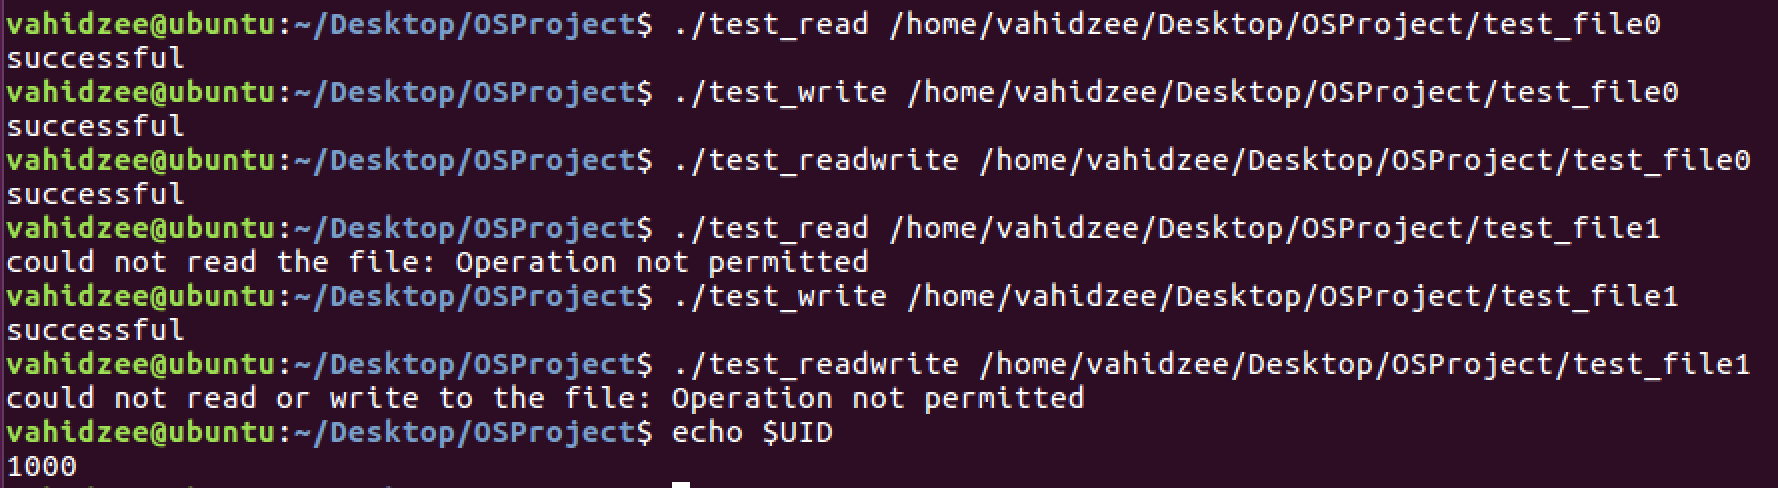
\includegraphics[width=0.8\textwidth]{screenshots/user(0)-cmds.png}
		\caption{حاصل اجرای کدهای تست برای کاربر ۱۰۰۰}
	\end{figure}

سپس با استفاده از دستور \texttt{su} کاربر به کاربر ۱۰۰۱ که دارای سطح دسترسی ۱ می‌باشد تغییر می‌کند. پس از  این دستور تعدادی خطای \texttt{bash} 
	رخ می‌دهد که دلیل آن سعی دستور \texttt{su} در نوشتن بر تعدادی فایل است که به دلیل سطح دسترسی بالاتر کاربر (۱ در برابر پیشفرض ۰ برای فایل‌ها) این عملیات غیر مجاز تلقی می‌شود. پس از آن سه کد مذکور بر روی دو فایل اجرا شدند. هر سه کد برای فایل دوم بدون مشکل اجرا شدند چرا که دارای سطحی برابر با سطح کاربر می‌باشند اما برای فایل اول تنها اجازه عملیات خواندن صادر شد.
      \begin{figure}[h]
      	\centering
      	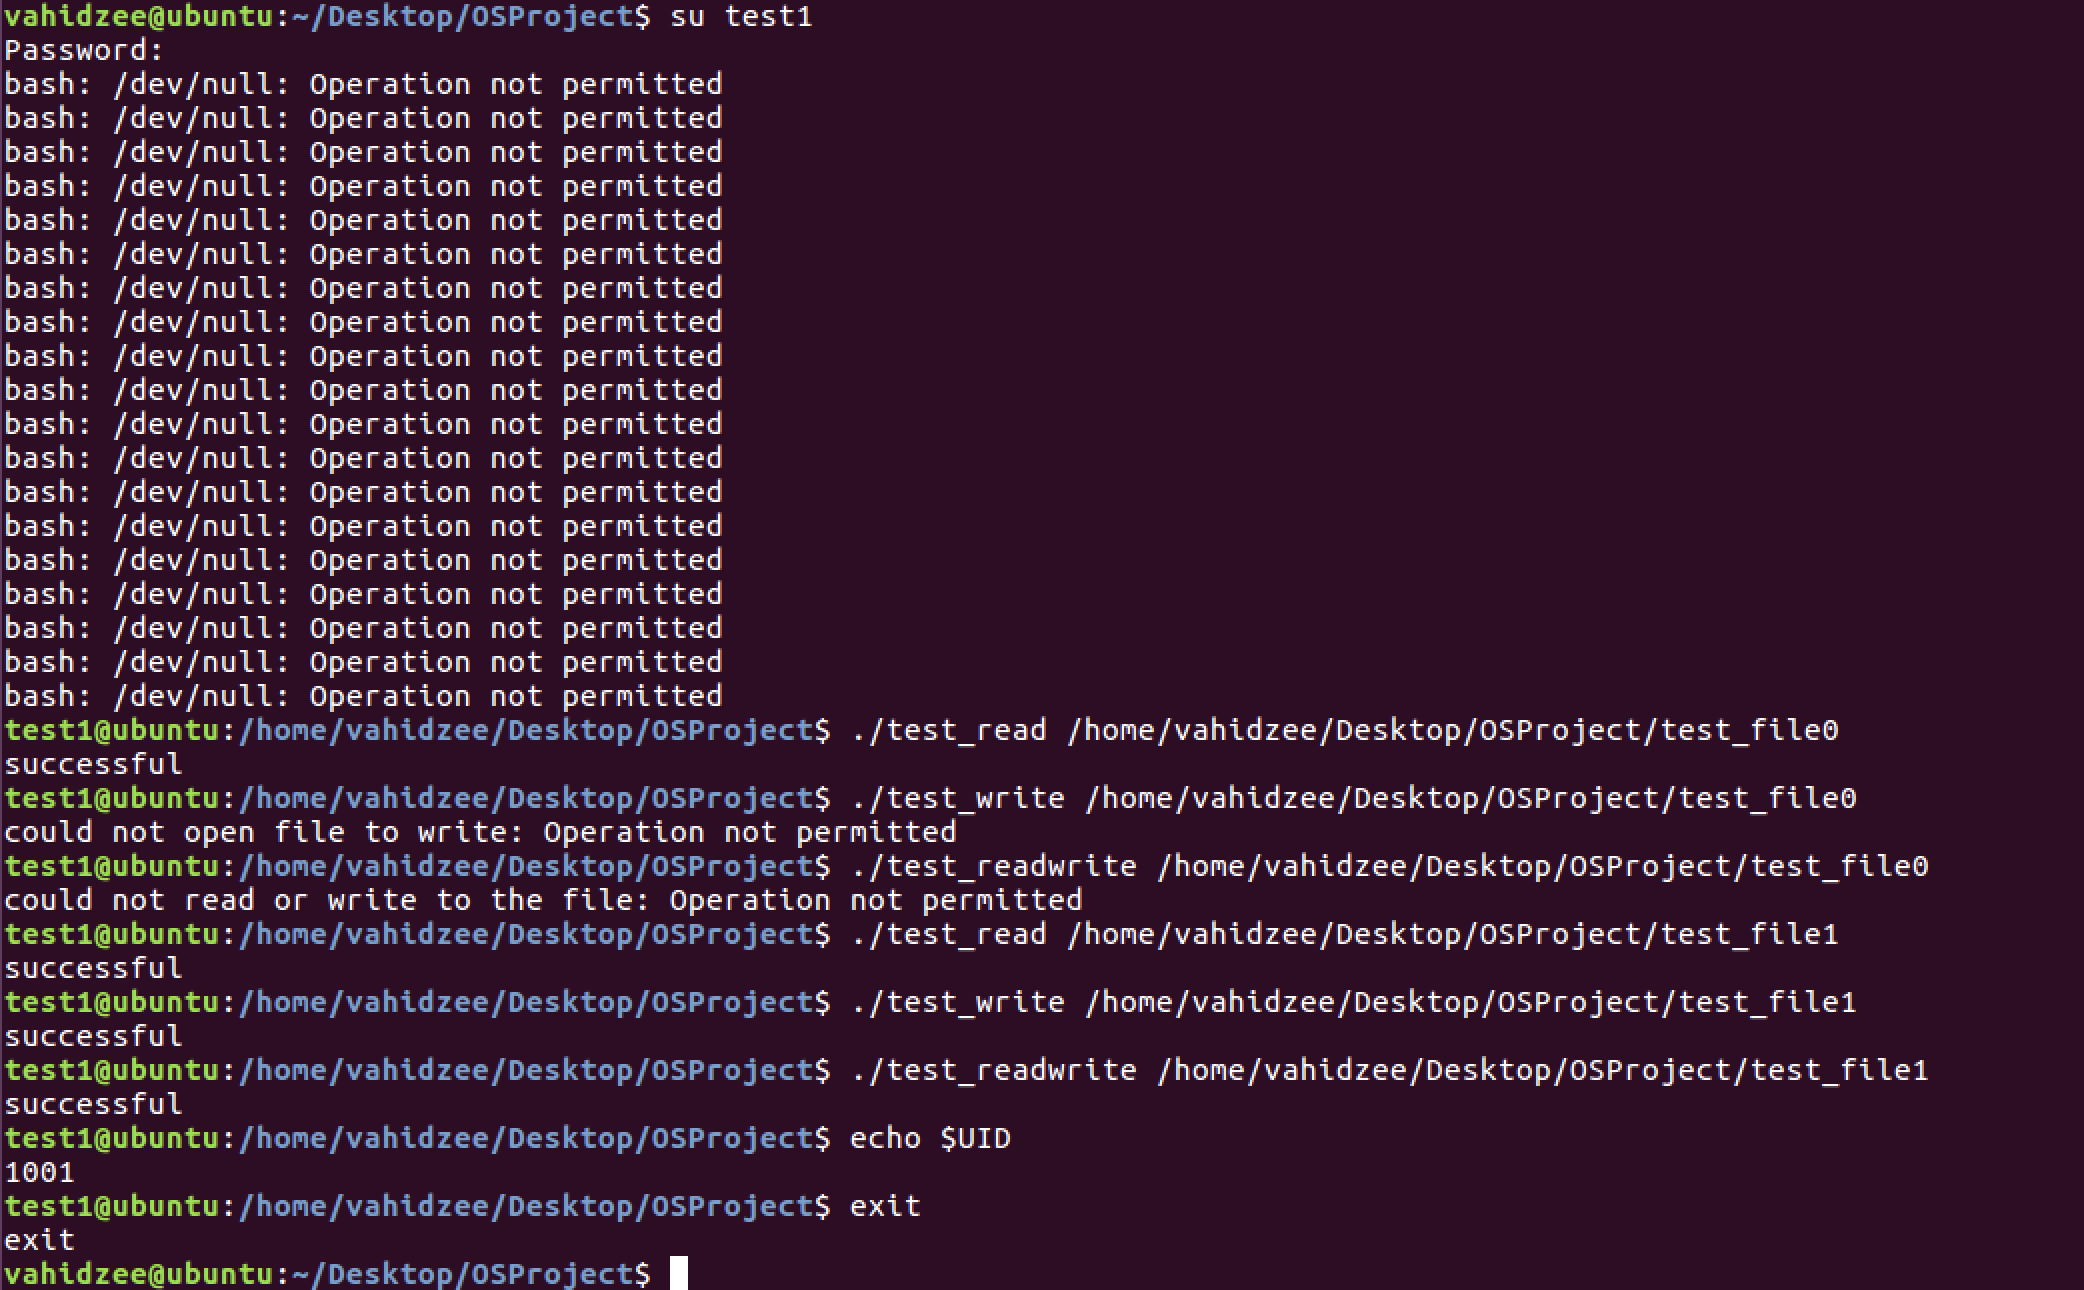
\includegraphics[width=0.8\textwidth]{screenshots/user(1)-cmds.png}
      	\caption{حاصل اجرای کدهای تست برای کاربر ۱۰۰۱}
      \end{figure}
  
  در نهایت همانند قبل به کاربر ۱۰۰۲ که دارای سطح دسترسی ۳ است تغییر صورت گرفت. این بار نیز مانند قبل خطاهای \texttt{bash} تولید شدند. حاصل اجرای کد نیز بر هر دو فایل نتیجه‌ی یکسانی در بر داشت؛ از آنجایی که سطح دسترسی این کاربر از هردو فایل بیشتر است، تنها عملیات خواندن با موفقیت انجام شد.
  \begin{figure}[h]
  	\centering
  	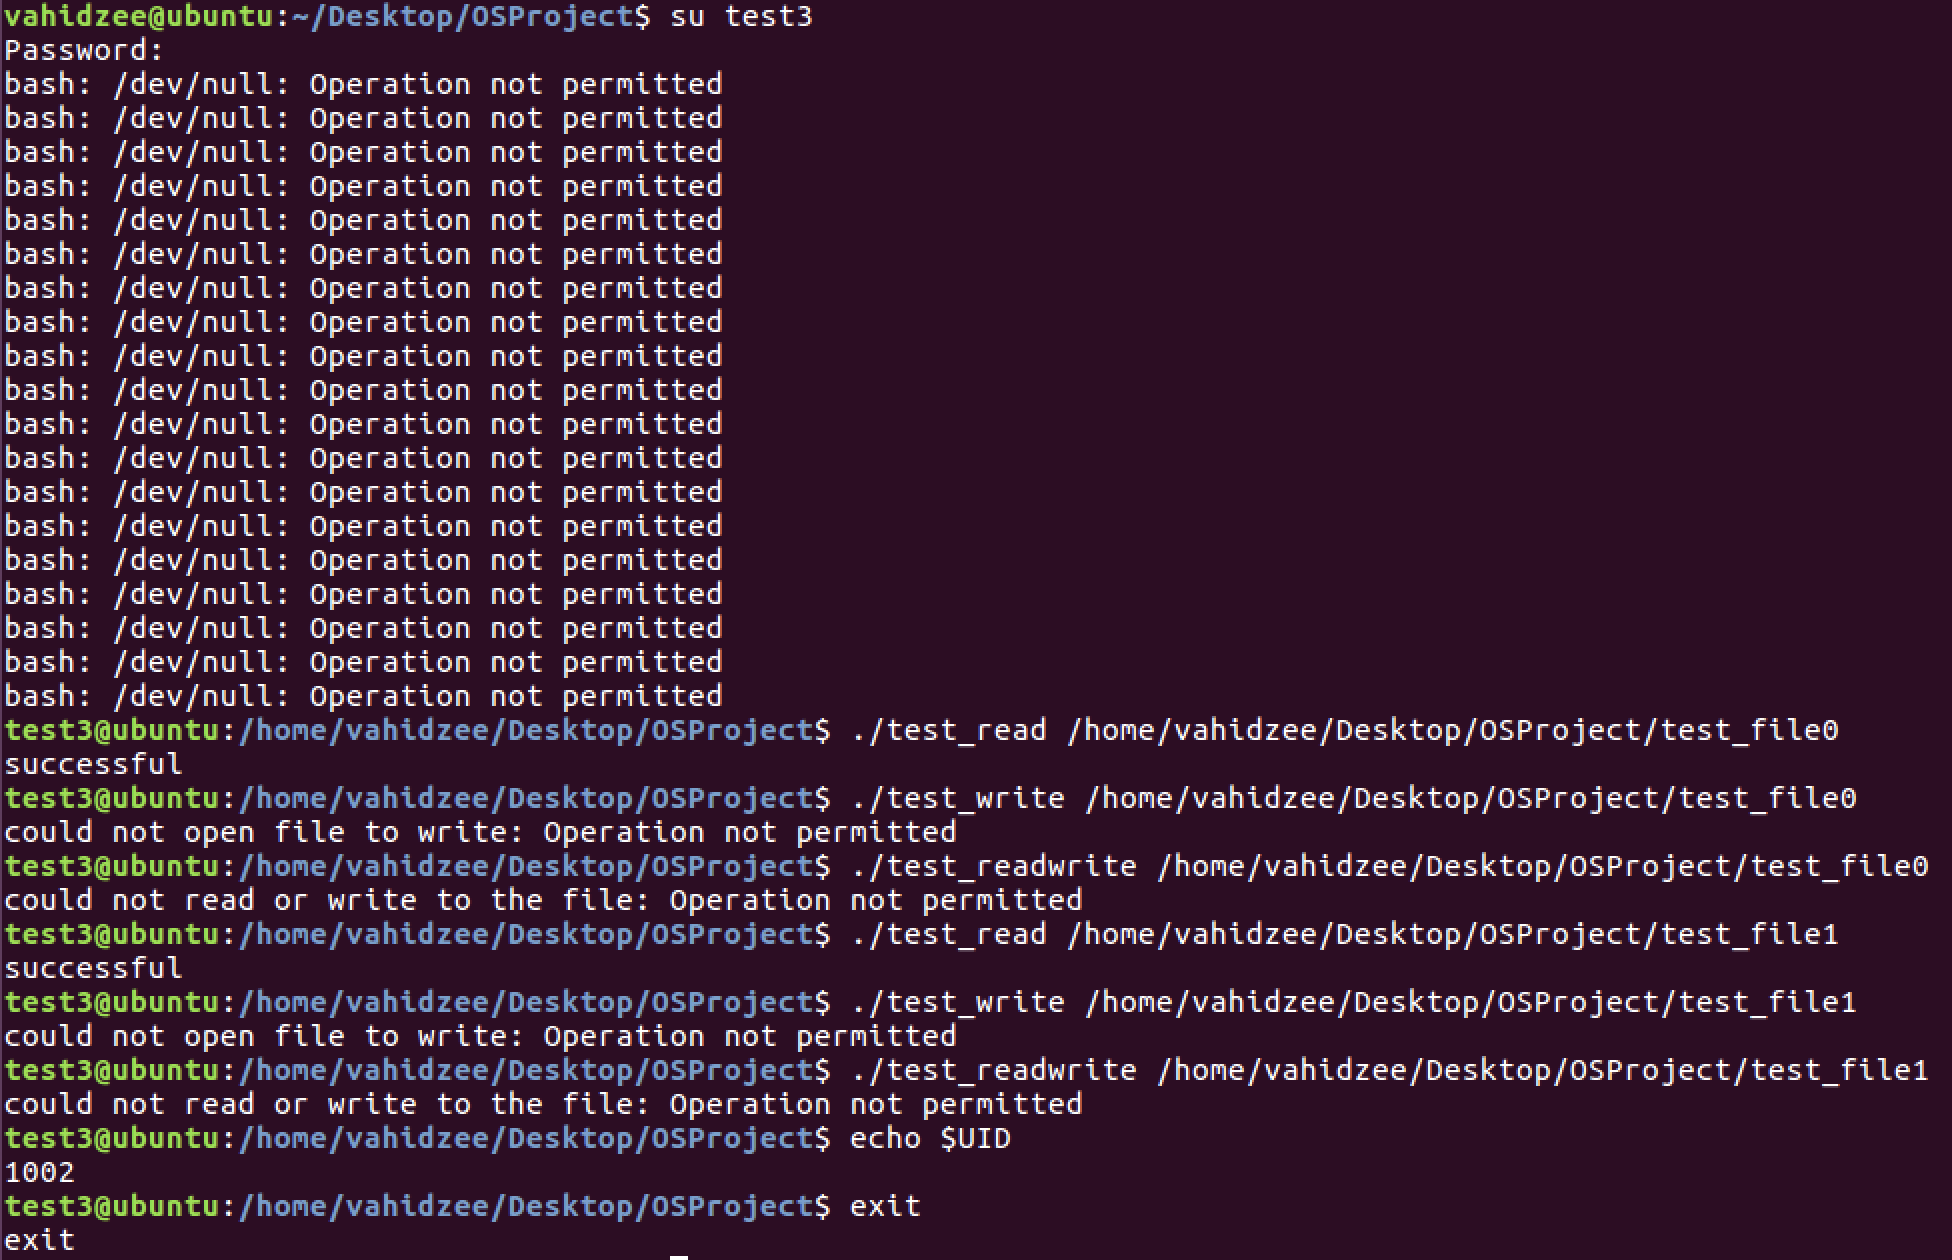
\includegraphics[width=0.8\textwidth]{screenshots/user(3)-cmds.png}
  	\caption{حاصل اجرای کدهای تست برای کاربر 1002}
  \end{figure}
  
  	در ادامه \lr{log}های ماژول در کرنل بررسی شدند تا عملکرد ماژول در قبال کاربرها و فایل‌هایی که مورد امتحان قرار گرفت تایید شوند. همچنین گزارشاتی که ماژول بر فایل می‌نویسد نیز بررسی شدند (بخش ۱.۵). فرمت این گزارشات به صورت ‫[شناسه کاربر-سطح کاربر-آدرس فایل-سطح فایل-نوع دسترسی-زمان] است.
  	\begin{figure}[h]
  		\centering
  		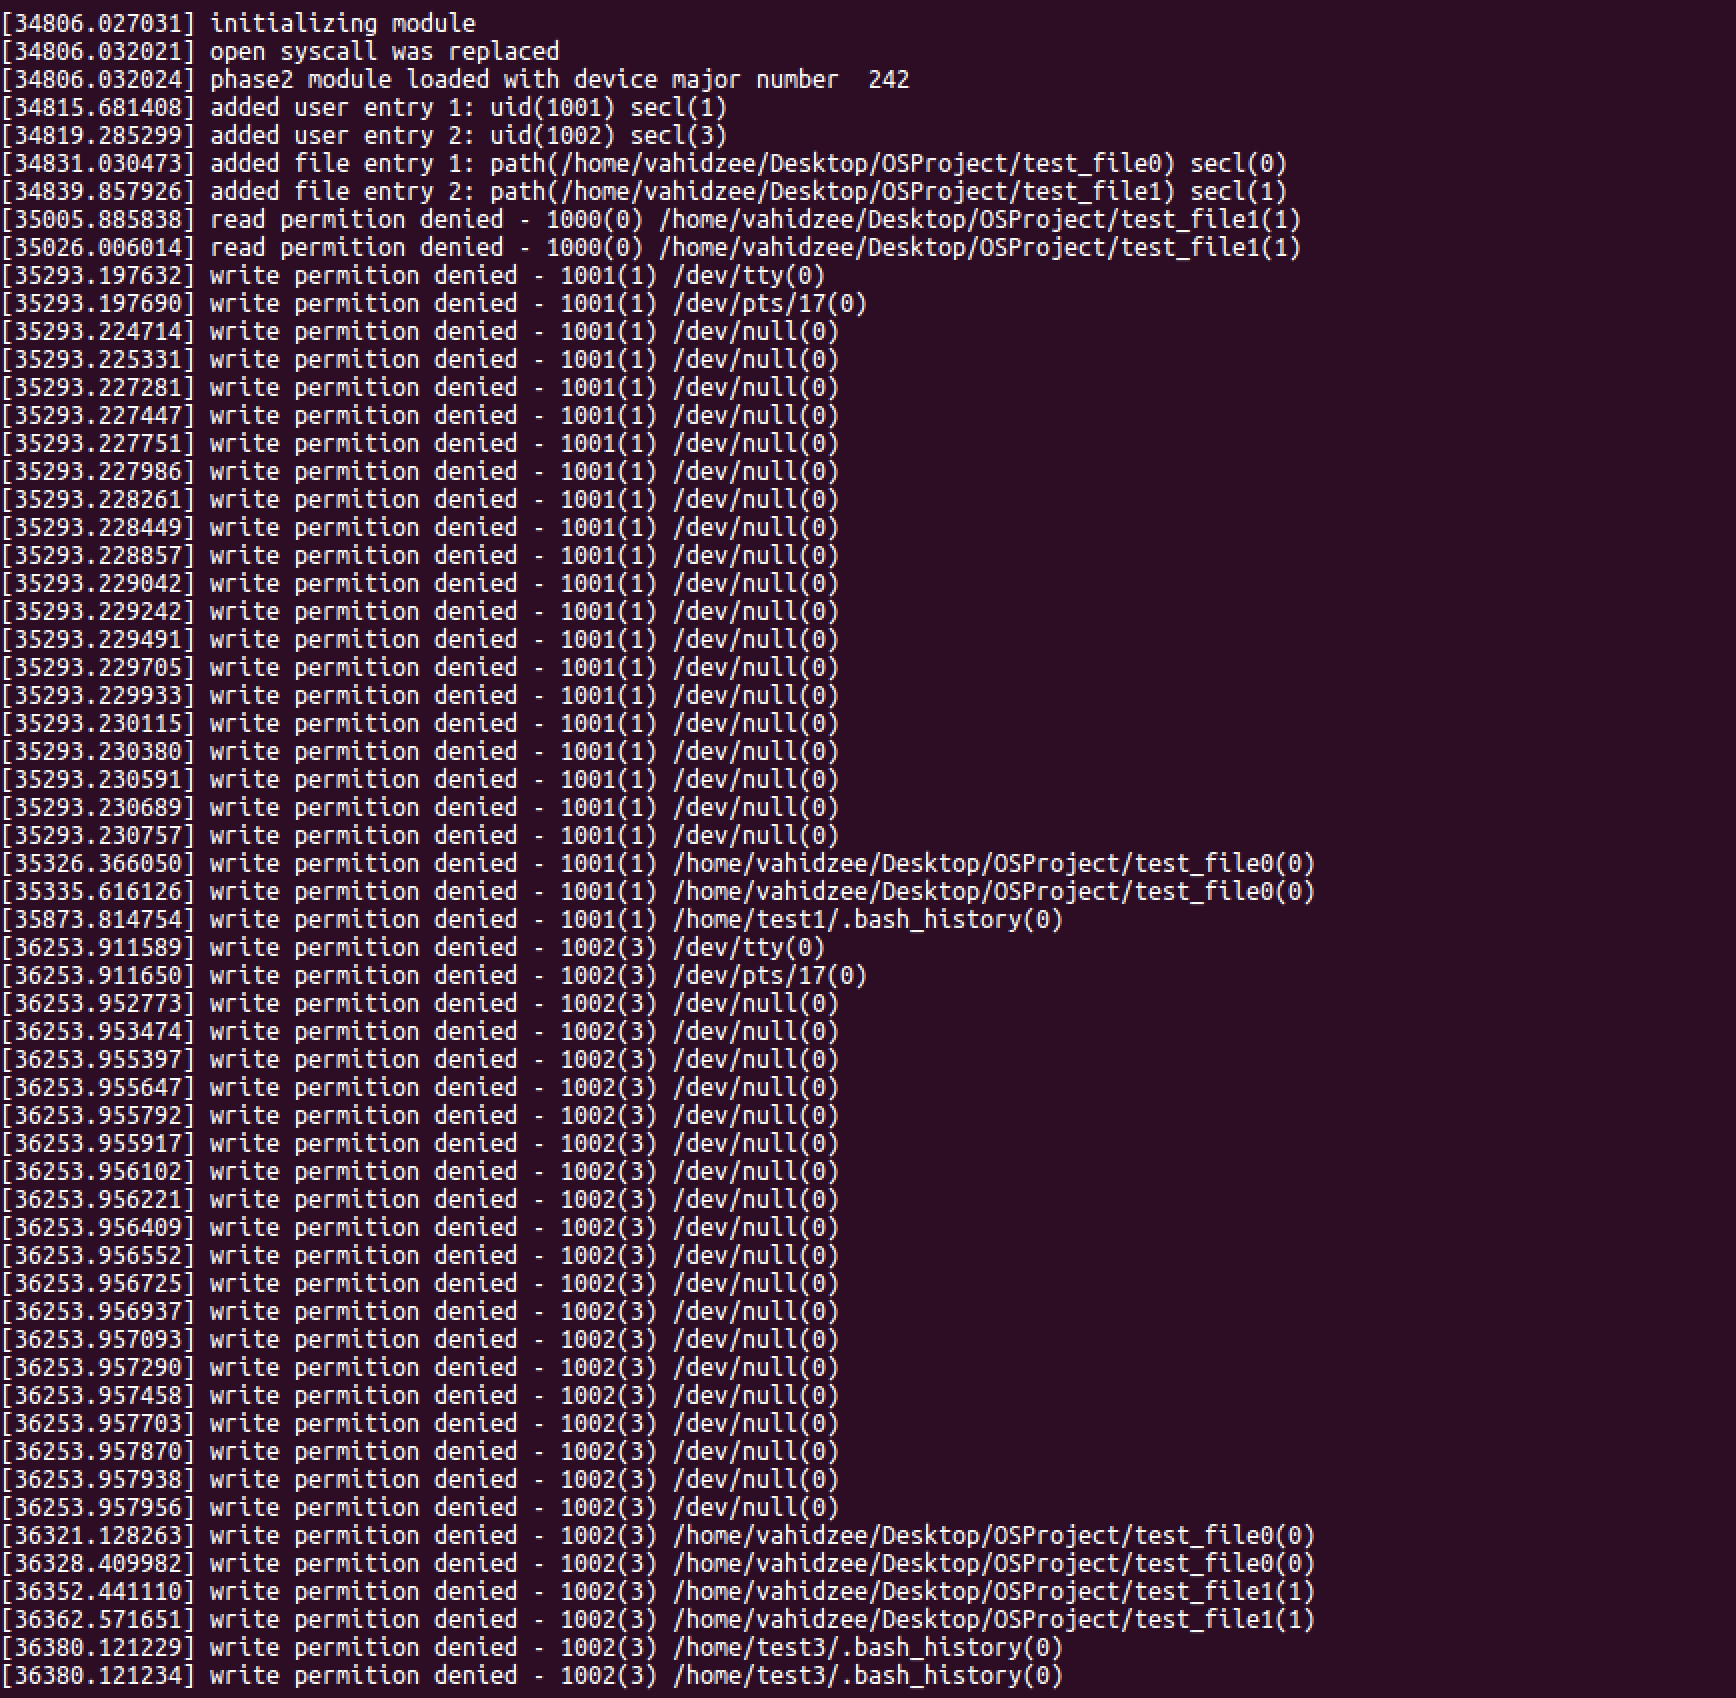
\includegraphics[width=0.8\textwidth]{screenshots/user(3)-kernel-log.png}
  		\caption{\lr{log}های ماژول در کرنل}
  	\end{figure}
  
  سه خط اول مربوط به افزودن ماژول به کرنل است. چهار خط بعدی مربوط به اضافه کردن کاربران و فایل‌ها به ماژول است و پس از آن دو خط آمده‌اند که نشانگر خطا هنگام دسترسی کاربر با سطح ۰ به فایل سطح ۱ برای خواندن/نوشتن و نوشتن می‌باشند. پس از آن نیز خطوط خطای \texttt{bash} و دسترسی 	
  	غیرمجاز دو کاربر دیگر نمایش‌داده‌ شده‌است.
      \begin{figure}[h]
      	\centering
      	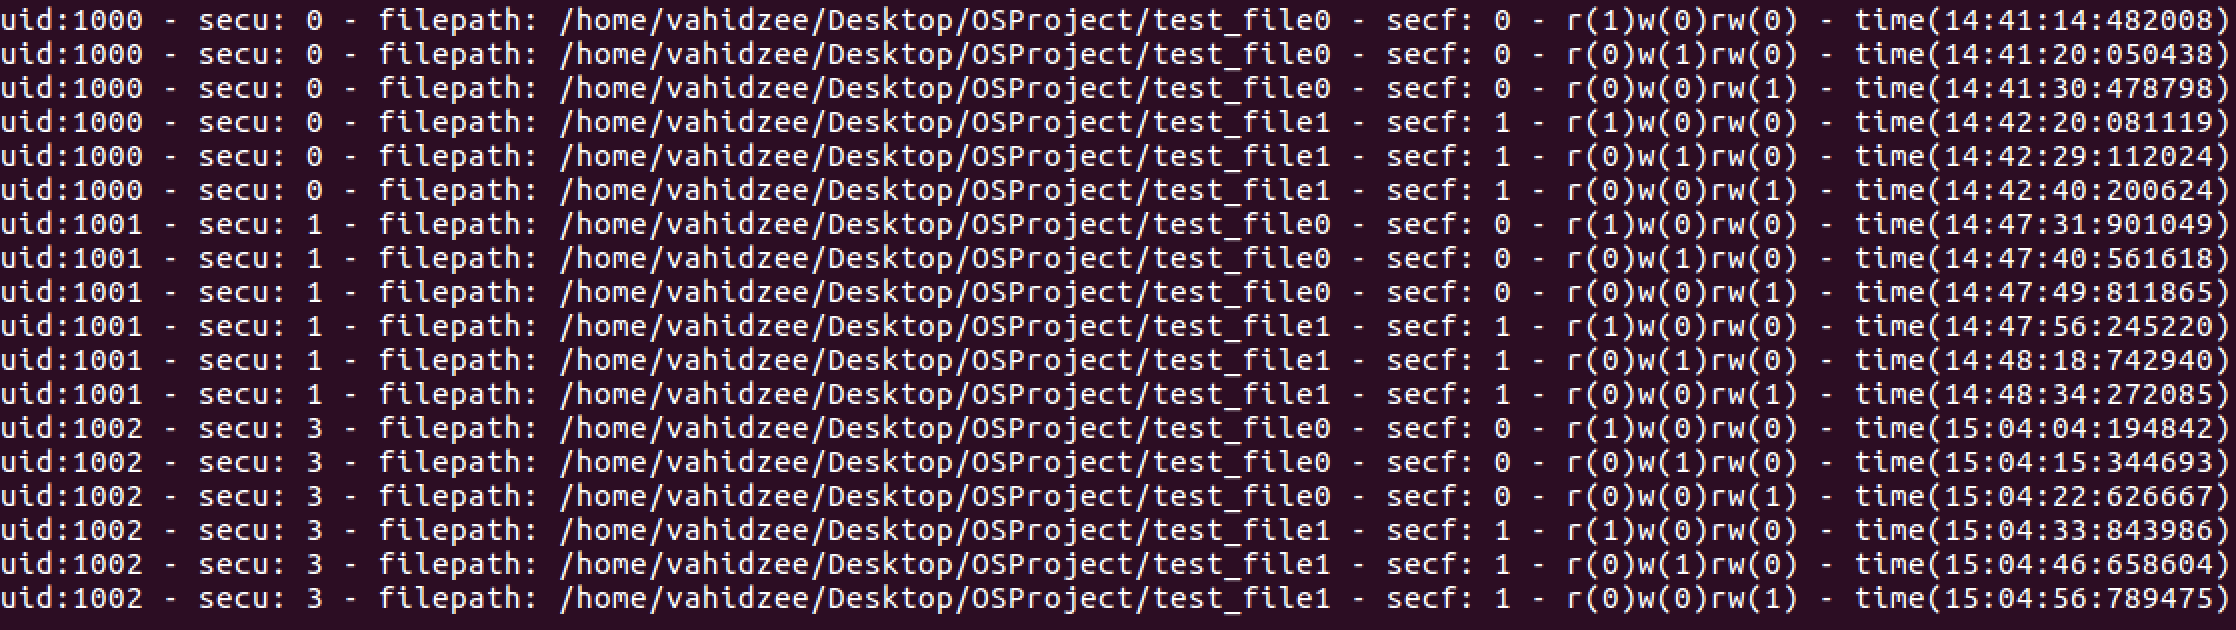
\includegraphics[width=0.8\textwidth]{screenshots/user(3)-access-log.png}
      	\caption{گزارشات ماژول}
      \end{figure}
  
  	در فایل گزارش نیز به ازای هر دسترسی یک 
  	\lr{log}
  	ثبت‌شده‌است که نوع هر دسترسی را دخیره می‌کند (خواندن: r - نوشتن: w - خواندن/نوشتن: rw ). بنابراین به تعداد ۳ کاربر $\times$
  	۲ فایل 
  	$\times$
  	۳ عملیات = ۱۸ خط گزارش خواهیم داشت.
  	\section{منابع}
  	\begin{latin}
  		\begin{itemize}
  			\item 
  			\href{https://stackoverflow.com/questions/59812156/how-can-i-override-a-system-call-table-entry-with-my-own-function}{How can I override a system call table entry with my own function?} 
  			\item
  			\href{https://stackoverflow.com/questions/58560284/linux-kernel-module-is-it-possible-to-use-an-open-function-inside-another-open}{Linux kernel module : Is it possible to use an open function inside another open function for my module?}
  			\item 
  			\href{https://man7.org/linux/man-pages/man2/open.2.html}{open(2) — Linux manual page}
  			\item 
  			\href{https://stackoverflow.com/questions/25719930/linux-kernel-logging-to-a-specific-file}{Linux kernel : logging to a specific file}
  			\item 
  			\href{https://stackoverflow.com/questions/5077192/how-to-get-current-hour-time-of-day-in-linux-kernel-space}{How to get current hour (time of day) in linux kernel space}
  	\end{itemize}
  	\end{latin}
  	
      
\end{document}    